\documentclass[twocolumns]{IEEEtran}
\usepackage{graphicx}
\usepackage{caption}
\usepackage{amsmath}
\graphicspath{{../figures/}}
\renewcommand\IEEEkeywordsname{Keywords}

\author{
	\IEEEauthorblockN{Erdal Sidal Dogan, Mert Komurcuoglu, Berkay Kurkcu} \\
	\IEEEauthorblockA{Facult of Engineering, MEF University \\
		Electrical \& Electronics Engineering Department}
}
\title{Audio Steganography}

\begin{document}
	\maketitle
	\begin{abstract}
		Digital Multimedia files such as images, videos, audio files etc. became ubiquitous in our lives. We can leverage these multimedia files for communication. Steganography is a technique for hiding information in these files in an imperceptible manner. By manipulating the multimedia signals, one can transmit messages to another in such a way that original signal would be indistinguishable from the manipulated one by a human. This paper demonstrates an application of audio steganography using MATLAB.
	\end{abstract}
	\begin{IEEEkeywords}
		Multimedia, steganography, signal.
	\end{IEEEkeywords}
	\section{Introduction}
	Steganography plays an important role in secret communication and data safety. There are many applications of steganography on different kinds of multimedia signals such as image, audio, video etc. along with multiple number of algorithms being used for similar purposes. In this project, we will be implementing the \textit{Least Significant Bit} algorithm on Audio signals using \textit{MATLAB}. Of course, there are multiple algorithms for similar purposes. However, after our researches we decided on LSB, since we don't need sophisticated needs such as fast encryption/decryption, higher amount of data transfer (bandwidth) etc, we considered the LSB would be an appropriate way to go. 
	
	
	\subsection{Literature Review}
	Data hiding in the least significant bits (LSBs) of
	audio samples in the time domain is one of the simplest
	algorithms with very high data rate of additional
	information . LSB coding  is one of the earliest
	techniques studied in the information hiding and
	watermarking area of digital audio (as well as other media
	types.  
	
	If we were to use more sophisticated methods we could use \textit{Threshold Based LSB} or \textit{Watermarking Method} algorithms. In \textit{Threshold Based LSB} method number of message bits changes depending on the amplitude of sampled signal\cite{threshold}. On the otherhand in \textit{Watermarking Method}, the LSB watermark encoder usually selects a subset and limits the number of of LSBs that can be imperceptibly modified during watermark embedding. The substitution operation on the LSBs is performed on this subset\cite{1286709}.
	
	
	Informations that we had from articles, we observed that,if
	16 bits per sample audio sequences are used,  the maximum LSB depth that
	can be used for LSB-based watermarking without causing
	noticeable perceptual distortion is the fourth LSB layer. According to the article, The tests
	were performed with a large collection of audio samples
	and individuals with different backgrounds and musical
	experience.
	
	\section{Method}
	Audio signals consist of thousands of samples which are represented as numerical values. As one can tell, all the numerical values are being stored in binary format by our computers. The binary format consist of 1's and 0's only. By looking at the positions of these 0 and 1's, we can get a decimal number. Right most digit of a binary number corresponds to $2^0$, as you move from right to left, power of 2 increases by 1. By adding the numbers shown as powers of 2 at where the bits on that position is 1, you can get a decimal number.
	\begin{figure}[h]
		\centering
		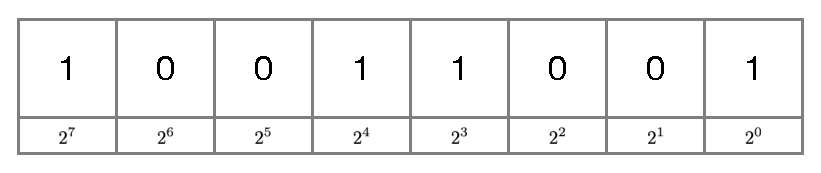
\includegraphics[scale=.5]{binary_num.eps}
		\caption{A binary number}
		\label{fig:binary}
	\end{figure}

	Figure \ref{fig:binary} shows the number $2^7 + 2^4 + 2^3 + 2^0 = 153$. As you can tell, the right-most bit of any binary number has a little effect on its decimal correspondent. For this example, if we flip the last bit from 1 to 0, decimal number would be equal to 152. Therefore, we can conclude that the right-most bit is the \textit{Least Significant Bit} of any binary number.
	
	The \textit{Least Significant Bit Algorithm} leverages this property of binary numbers for hiding messages in a audio file. As stated earlier, audio files consists samples that are represented by decimal number. Now, let's think about a sequence of an audio signal, assume it goes by; (normalized between -1 and 1)\\
	\begin{equation}
	\begin{bmatrix}
		0.143 & -0.471 & 0.643 & \hdots \\
	\end{bmatrix}
	\end{equation}
	The samples can be multiplied with a greater number to become integer values because the precision numbers representations are more complex than integer. Our input signal was decoded with 16 bits per sample. Thus, we multiplied each sample with $2^{15} = 32768$ for them to become integers that can be represented by 16 bits.
	\begin{equation}
		\begin{bmatrix}
		'000000000110011' \\
		'000000000000000' \\
		'000000000011000' \\
		'000000110100001' \\
		\vdots
		\end{bmatrix} \\ \\		
	\end{equation}
	\begin{center}
		Actual first 4 sample of the audio file
	\end{center}

	
	\section{Implementation}
	The program has been implemented on \textit{MATLAB} as a necessity of the course and its competency on processing media signals.
	
	\bibliographystyle{IEEEtran}
	\bibliography{references.bib}

\end{document}